
% ════════════════════════════════════════════
% 模型求解（5.3.4.模型求解.tex，三级子块）
% ════════════════════════════════════════════
\subsubsection{调整收益与边际价值分析}

基于上述模型，本节在 0:00、6:00、12:00、18:00 四个预报时刻顺序求解四个线性规划。以 1 月为预热期、费用汇总仅统计 2 月 1 日—12 月 31 日（334 天），含调整的总购电费用为 14337999.15 元；不引入调整、仅执行 0:00 计划时为 14782072.51 元，滚动调整降低费用 444073.36 元，降幅约 3.00\%。按题目要求的表 1—表 3 格式，四个指定日期的计划与调整结果汇总于表\ref{tab:结果3-1}，储能充放电量见表\ref{tab:结果3-2}（四个指定日 0:00 与 24:00 的储电量均为 1200.00 kWh，即储能下限），各日紧急购电分段见表\ref{tab:结果3-3}。

{\footnotesize\renewcommand{\arraystretch}{0.95}\begin{longtable}{>{\centering\arraybackslash}p{0.22\textwidth}>{\centering\arraybackslash}p{0.155\textwidth}>{\centering\arraybackslash}p{0.155\textwidth}>{\centering\arraybackslash}p{0.155\textwidth}>{\centering\arraybackslash}p{0.155\textwidth}}
  
  \caption{2025 年四个典型日在指定时间段的计划购电量、全天计划与调整购电量（kWh）及全天计划与紧急购电费（元）}
  \label{tab:结果3-1}\label{tab:结果3-4} \\
  \toprule
  项目 & 2025.3.20 & 2025.6.21 & 2025.9.23 & 2025.12.21 \\
  \midrule
  \endfirsthead
  \caption{2025 年四个典型日在指定时间段的计划购电量、全天计划与调整购电量（kWh）及全天计划与紧急购电费（元）（续）} \\
  \toprule
  项目 & 2025.3.20 & 2025.6.21 & 2025.9.23 & 2025.12.21 \\
  \midrule
  \endhead
  \bottomrule
  \endfoot
  10:00--10:10 & 0.00 & 0.00 & 0.00 & 0.00 \\
  12:00--12:10 & 560.43 & 0.00 & 371.59 & 979.54 \\
  14:00--14:10 & 0.00 & 0.00 & 0.00 & 0.00 \\
  16:00--16:10 & 663.99 & 111.20 & 636.70 & 799.69 \\
  18:00--18:10 & 698.00 & 0.00 & 764.33 & 715.41 \\
  20:00--20:10 & 0.00 & 0.00 & 0.00 & 0.00 \\
  全天计划购电量 & 67748.70 & 32640.60 & 68433.20 & 93633.20 \\
  全天调整购电量 & 63217.60 & 33140.10 & 65716.30 & 93783.50 \\
  全天计划购电费 & 41072.00 & 18056.00 & 42736.00 & 59704.00 \\
  全天紧急购电费 & 12856.00 & 2294.00 & 5600.00 & 2875.00 \\
\end{longtable}}

\begin{table}[H]
  \centering
  \footnotesize
  \renewcommand{\arraystretch}{0.95}
  \caption{2025 年四个典型日（问题三）储能设备在指定时间段的充放电量（kWh），及四个典型日 0:00 与 24:00 的储电量（kWh）}
  \label{tab:结果3-2}
  \begin{tabular}{>{\centering\arraybackslash}p{0.125\textwidth}*{8}{>{\centering\arraybackslash}p{0.098\textwidth}}}
  \toprule
  \multirow{2}{*}{时间段} & \multicolumn{2}{c}{2025.3.20} & \multicolumn{2}{c}{2025.6.21} & \multicolumn{2}{c}{2025.9.23} & \multicolumn{2}{c}{2025.12.21} \\
  \cmidrule(lr){2-3}\cmidrule(lr){4-5}\cmidrule(lr){6-7}\cmidrule(lr){8-9}
   & 充电量 & 放电量 & 充电量 & 放电量 & 充电量 & 放电量 & 充电量 & 放电量 \\
  \midrule
  0:00--4:00 & 9000.00 & 0.00 & 1409.41 & 0.00 & 9000.00 & 0.00 & 9000.00 & 0.00 \\
  4:00--8:00 & 1666.67 & 6149.96 & 850.39 & 1830.44 & 1666.67 & 6435.18 & 2499.34 & 1510.13 \\
  8:00--12:00 & 4106.95 & 2313.92 & 1812.59 & 0.00 & 5210.49 & 1920.52 & 5833.33 & 7579.05 \\
  12:00--16:00 & 6651.73 & 250.65 & 8722.90 & 0.00 & 5495.20 & 315.91 & 7558.00 & 2432.26 \\
  16:00--20:00 & 0.00 & 5709.78 & 131.18 & 6154.10 & 0.00 & 5602.91 & 0.00 & 5797.47 \\
  20:00--24:00 & 0.00 & 2930.22 & 0.00 & 2485.90 & 0.00 & 3037.09 & 0.00 & 2842.53 \\
  0:00 储电量 & \multicolumn{2}{c}{1200.00} & \multicolumn{2}{c}{1200.00} & \multicolumn{2}{c}{1200.00} & \multicolumn{2}{c}{1200.00} \\
  24:00 储电量 & \multicolumn{2}{c}{1200.00} & \multicolumn{2}{c}{1200.00} & \multicolumn{2}{c}{1200.00} & \multicolumn{2}{c}{1200.00} \\
  \bottomrule
  \end{tabular}
\end{table}

{\footnotesize\renewcommand{\arraystretch}{0.95}\begin{longtable}{>{\centering\arraybackslash}p{0.11\textwidth}>{\centering\arraybackslash}p{0.08\textwidth}>{\centering\arraybackslash}p{0.11\textwidth}>{\centering\arraybackslash}p{0.08\textwidth}>{\centering\arraybackslash}p{0.11\textwidth}>{\centering\arraybackslash}p{0.08\textwidth}>{\centering\arraybackslash}p{0.11\textwidth}>{\centering\arraybackslash}p{0.08\textwidth}}
  
  \caption{微网在指定日期的紧急购电量}
  \label{tab:结果3-3} \\
  \toprule
  \multicolumn{2}{c}{2025.3.20} & \multicolumn{2}{c}{2025.6.21} & \multicolumn{2}{c}{2025.9.23} & \multicolumn{2}{c}{2025.12.21} \\
  \cmidrule(lr){1-2} \cmidrule(lr){3-4} \cmidrule(lr){5-6} \cmidrule(lr){7-8}
  时间段 & 购电量 & 时间段 & 购电量 & 时间段 & 购电量 & 时间段 & 购电量 \\
  \midrule
  \endfirsthead
  \caption{微网在指定日期的紧急购电量（续）} \\
  \toprule
  \multicolumn{2}{c}{2025.3.20} & \multicolumn{2}{c}{2025.6.21} & \multicolumn{2}{c}{2025.9.23} & \multicolumn{2}{c}{2025.12.21} \\
  \cmidrule(lr){1-2} \cmidrule(lr){3-4} \cmidrule(lr){5-6} \cmidrule(lr){7-8}
  时间段 & 购电量 & 时间段 & 购电量 & 时间段 & 购电量 & 时间段 & 购电量 \\
  \midrule
  \endhead
  \bottomrule
  \endfoot
  06:00--12:00 & 2497.25 & 04:00--04:50 & 2.34 & 06:00--06:50 & 692.04 & 07:00--08:10 & 67.18 \\
  12:30--14:20 & 545.00 & 05:00--05:30 & 12.59 & 07:10--08:00 & 61.88 & 08:50--12:00 & 829.59 \\
  14:40--15:10 & 35.16 & 06:00--06:10 & 140.85 & 08:10--09:00 & 64.49 & 13:00--13:10 & 2.28 \\
  15:20--16:20 & 119.81 & 06:20--07:20 & 360.87 & 09:50--10:20 & 46.53 & 16:30--16:50 & 13.69 \\
  16:50--17:50 & 77.14 & 13:00--13:10 & 1.48 & 10:40--11:00 & 48.04 &  &  \\
   &  & 16:00--16:20 & 5.78 & 11:40--12:00 & 57.68 &  &  \\
   &  & 17:20--17:30 & 0.50 & 12:50--14:00 & 121.33 &  &  \\
   &  & 19:00--19:50 & 2.58 & 14:20--15:00 & 92.64 &  &  \\
   &  &  &  & 15:50--16:30 & 24.37 &  &  \\
   &  &  &  & 17:00--17:50 & 64.93 &  &  \\
\end{longtable}}

以 9 月 23 日为例（图\ref{fig:结果3-2}），调整后购电功率在光伏预报偏高的白天时段被下调，减少了高价时段的无效购电，预报偏低时则小幅上调，缩小供电缺口。逐日紧急购电量（图\ref{fig:结果3-3}）多数日期维持低位，仅在个别缺口日出现尖峰，说明调整已吸收大部分预报误差。

\begin{figure}[H]
    \centering
    \begin{minipage}[t]{0.46\textwidth}
        \centering
        \vspace{0pt}
        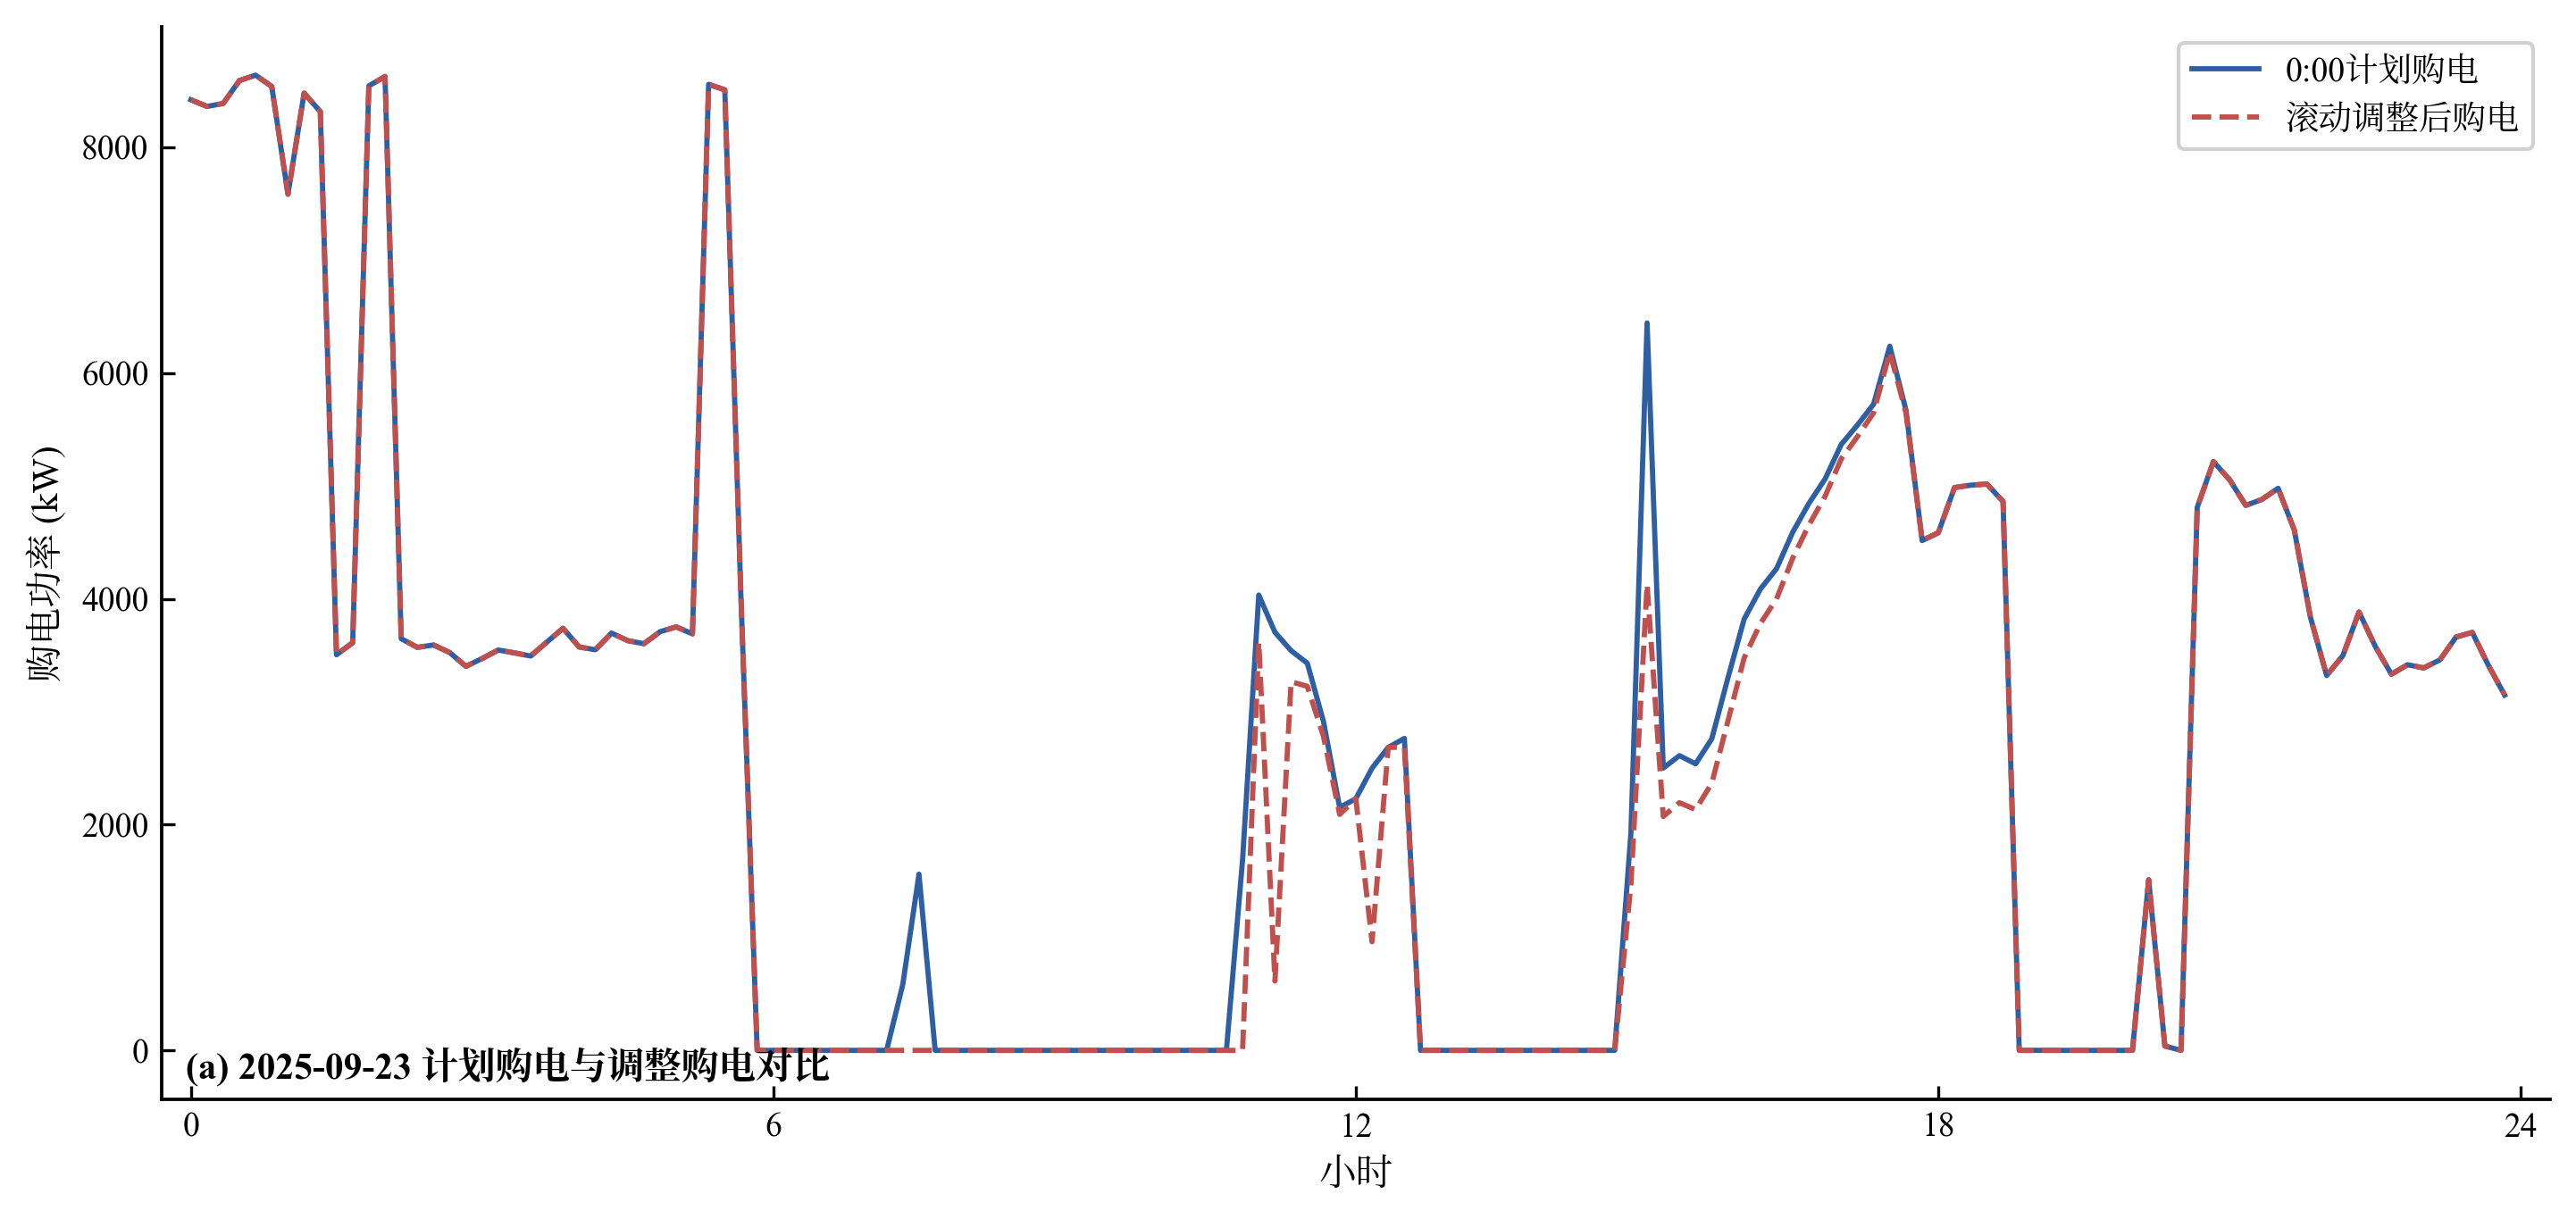
\includegraphics[width=\textwidth]{求解/问题三/图片/图3-2_计划与调整购电量对比.png}
        \caption{典型日计划购电与调整购电功率对比}
        \label{fig:结果3-2}
    \end{minipage}
    \hfill
    \begin{minipage}[t]{0.46\textwidth}
        \centering
        \vspace{0pt}
        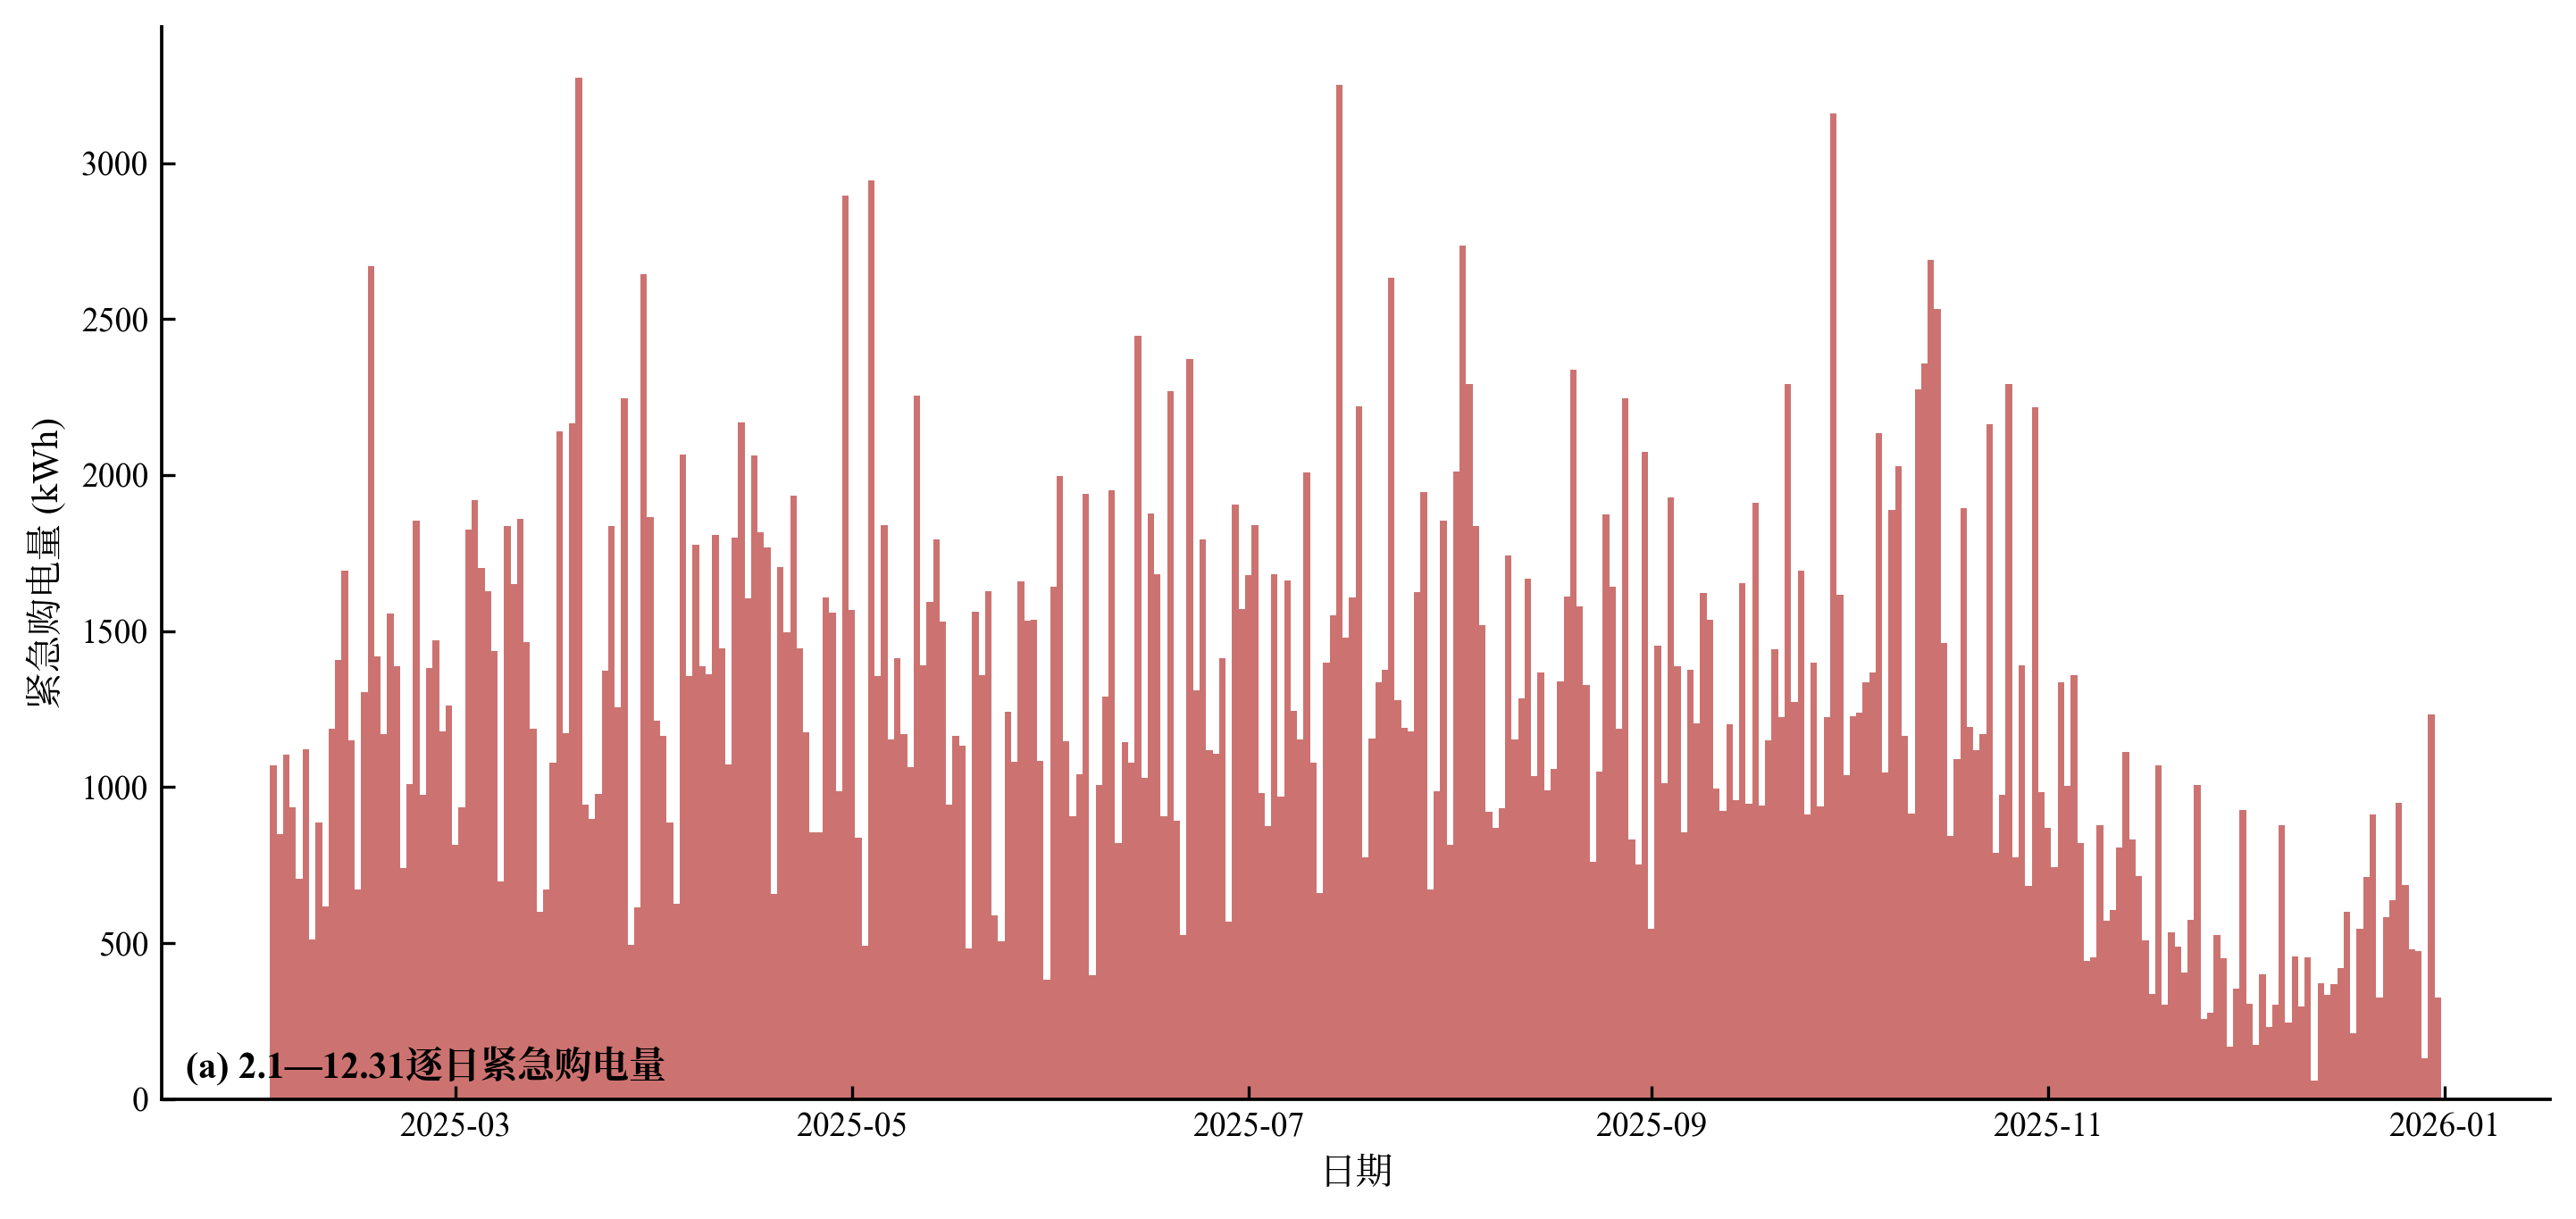
\includegraphics[width=\textwidth]{求解/问题三/图片/图3-3_全年紧急购电量.png}
        \caption{2.1—12.31逐日紧急购电量}
        \label{fig:结果3-3}
    \end{minipage}
\end{figure}

引入滚动调整后，总费用由 14782072.51 元降至 14337999.15 元，各月均有节省（图\ref{fig:结果3-4}），利用 6:00、12:00、18:00 预报调整购电具有经济收益。

\begin{figure}[H]
    \centering
    \begin{minipage}[t]{0.46\textwidth}
        \centering
        \vspace{0pt}
        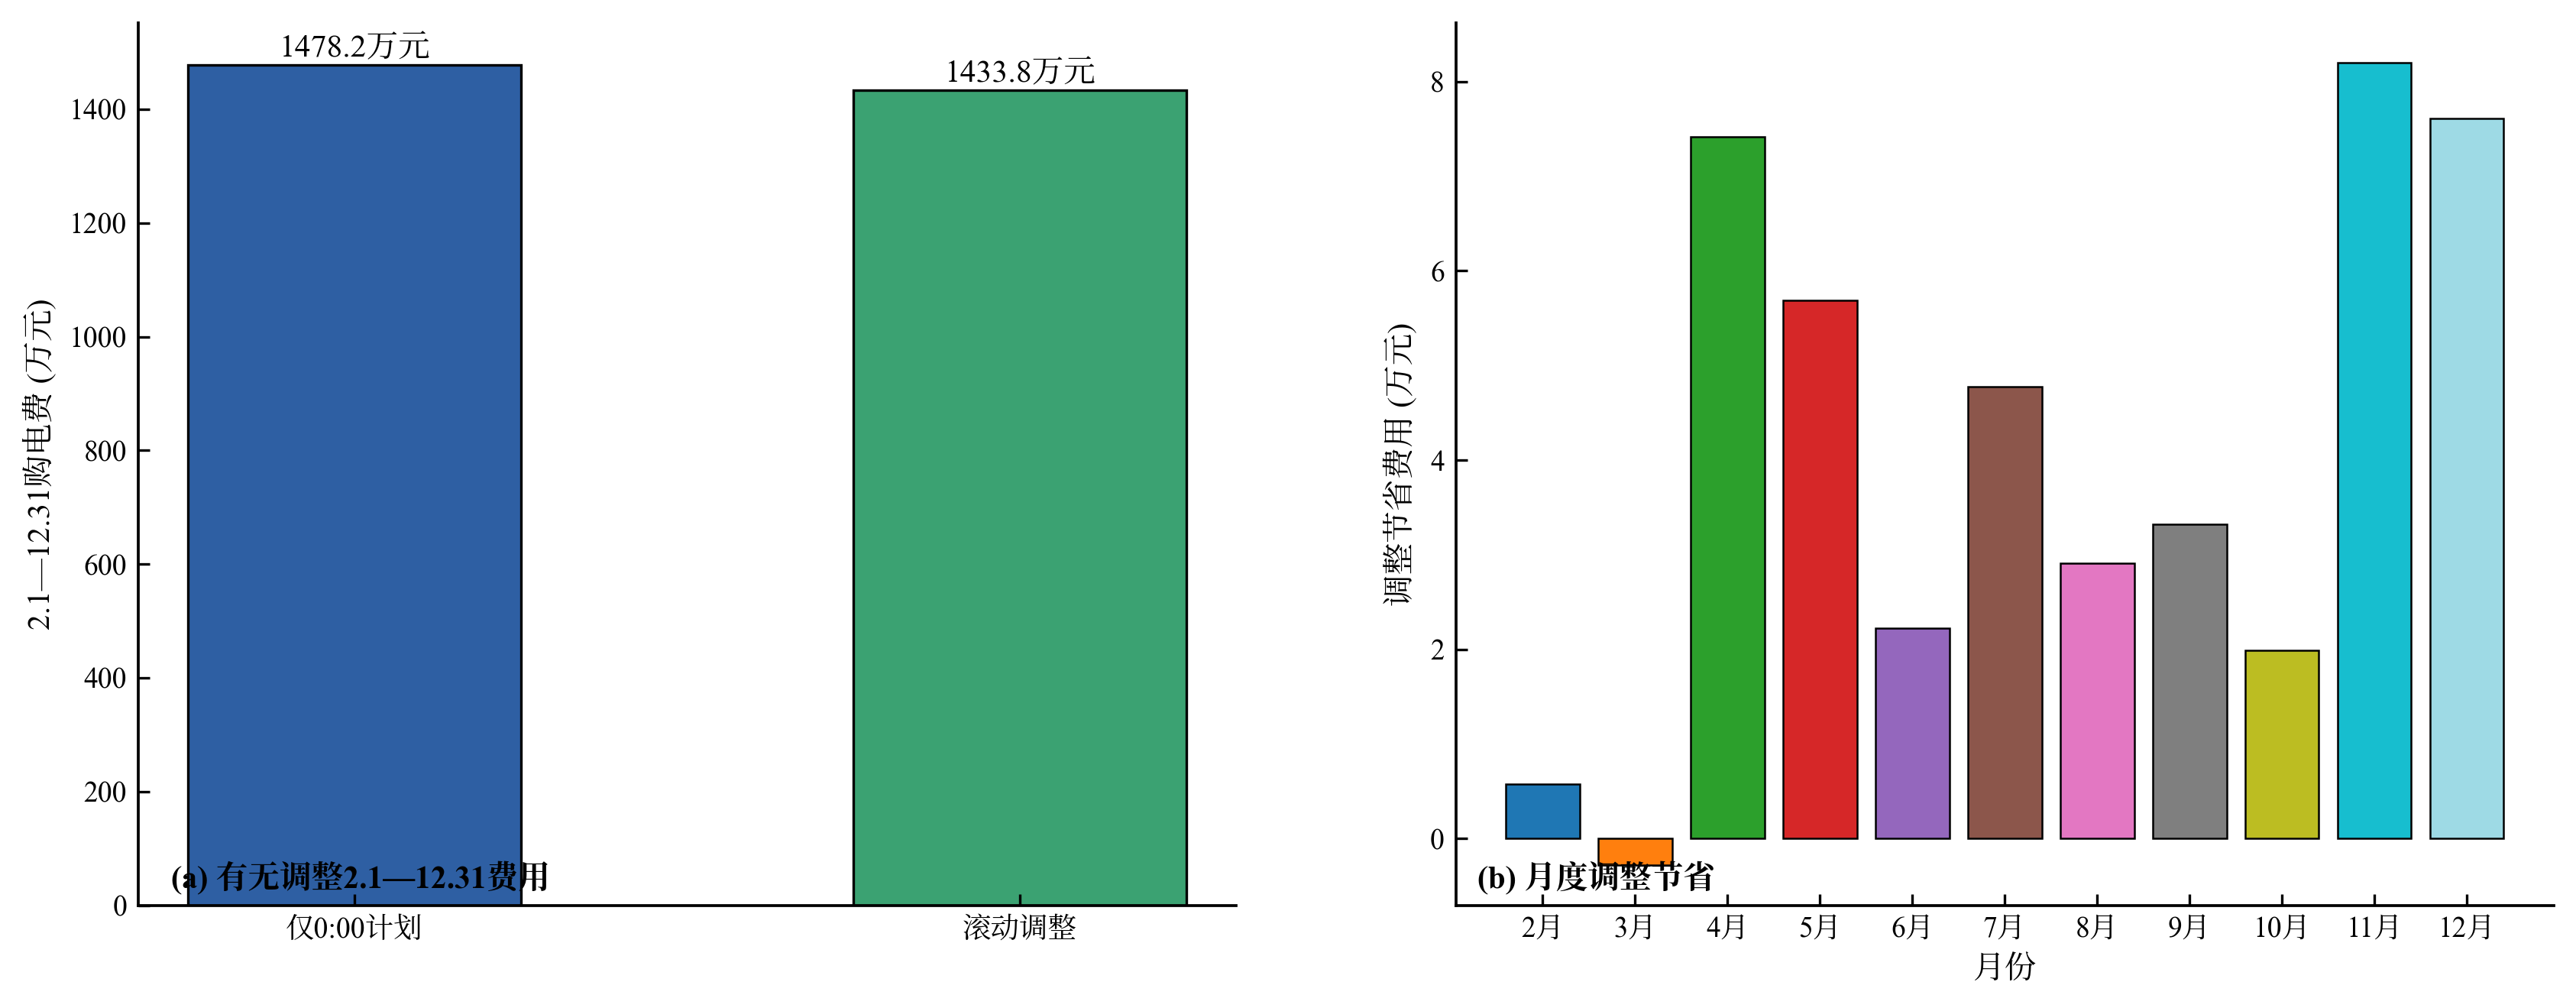
\includegraphics[width=\textwidth]{求解/问题三/图片/图3-4_有无调整费用对比.png}
        \caption{有无滚动调整的费用对比与月度节省（2.1—12.31）}
        \label{fig:结果3-4}
    \end{minipage}
    \hfill
    \begin{minipage}[t]{0.46\textwidth}
        \centering
        \vspace{0pt}
        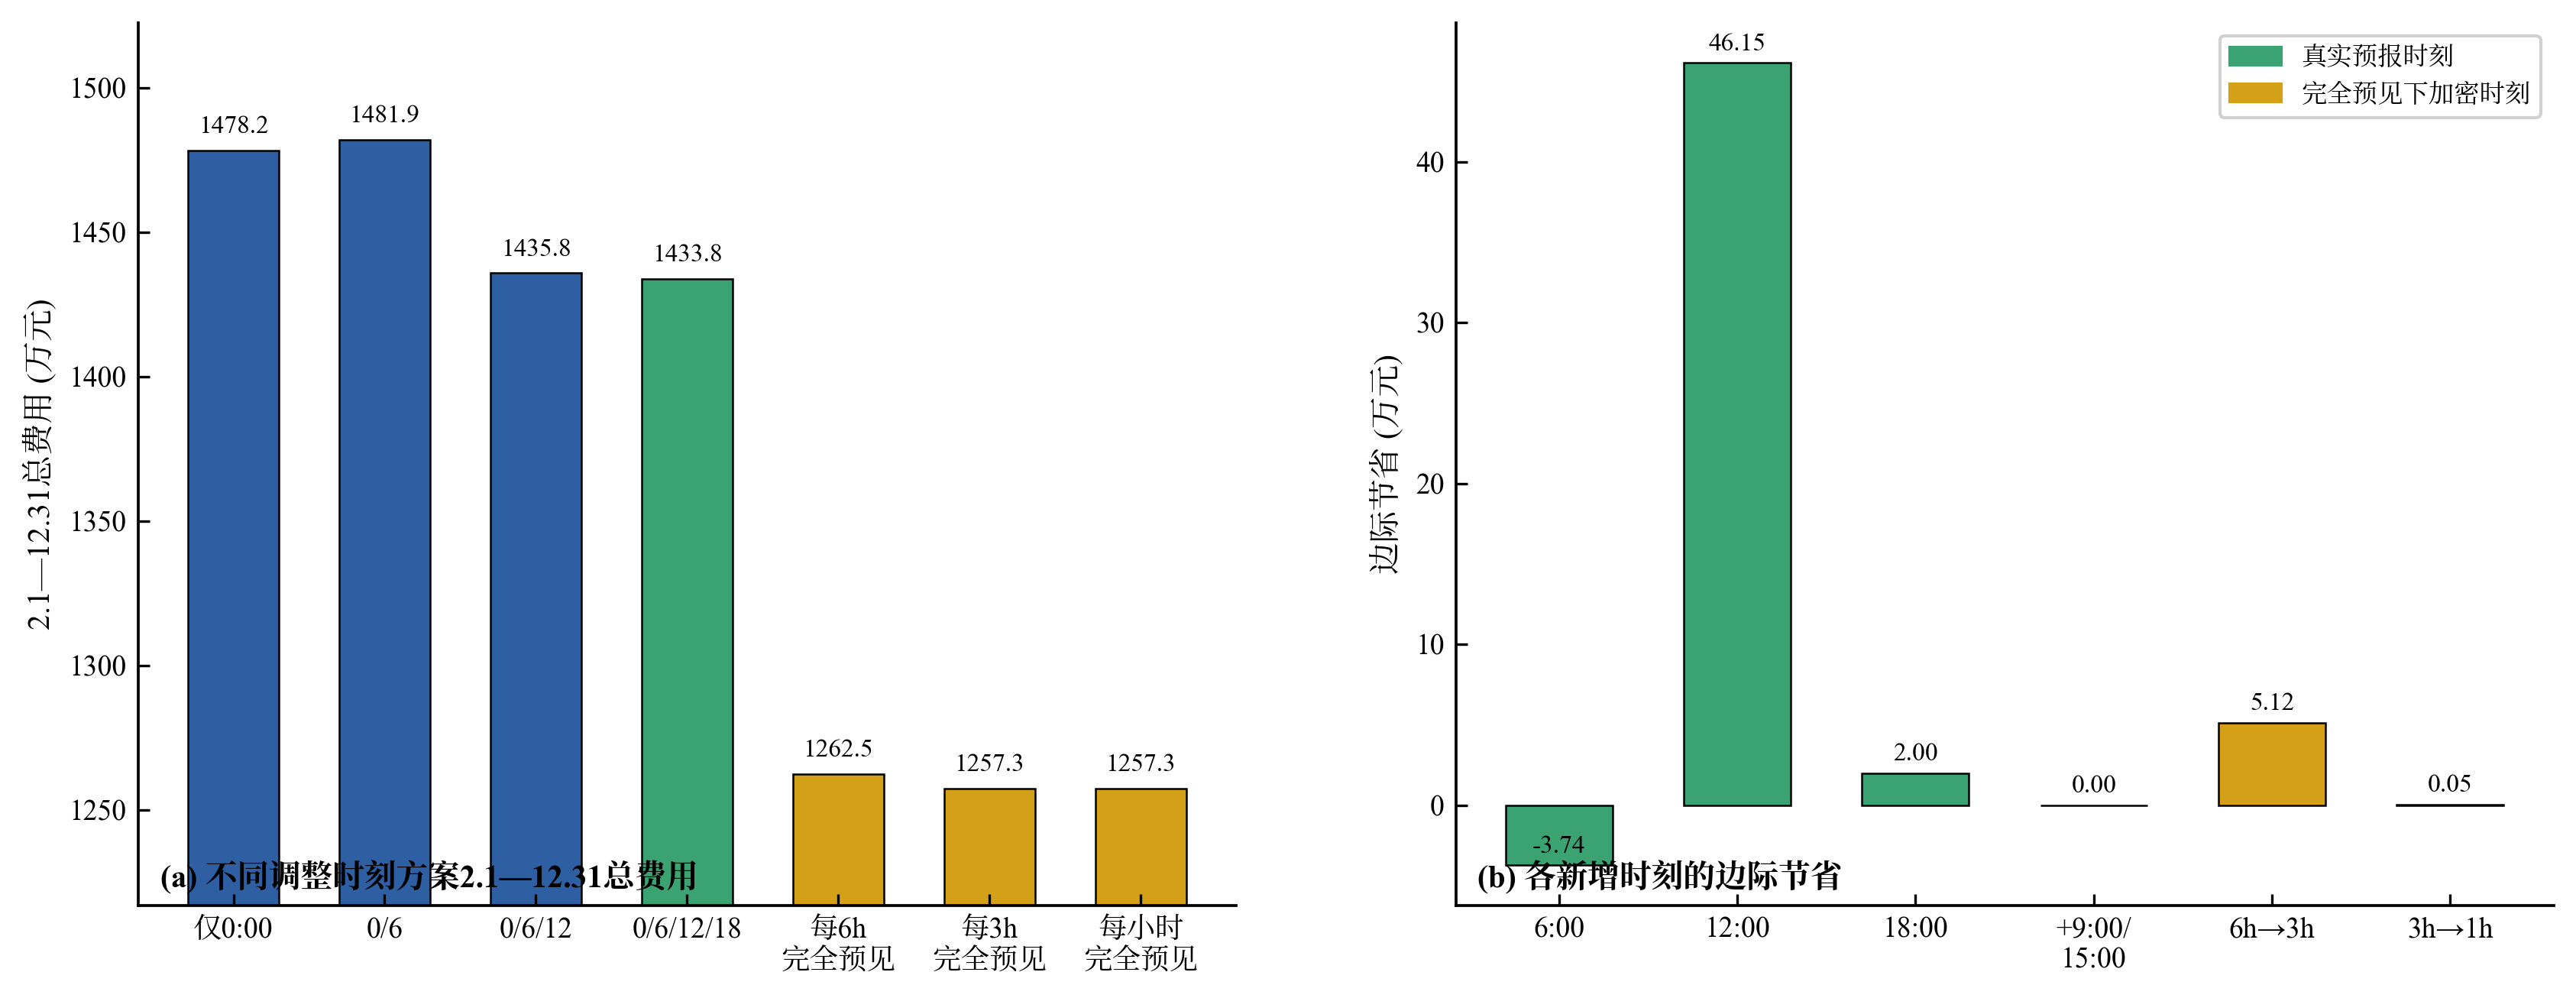
\includegraphics[width=\textwidth]{求解/问题三/图片/图3-7_其他时刻预报边际收益.png}
        \caption{不同调整时刻方案的总费用与各新增时刻的边际节省（2.1—12.31）}
        \label{fig:结果3-7}
    \end{minipage}
\end{figure}

储能荷电状态全程处于 $[1200,10800]$ kWh 约束区间内，调整策略在提升经济性的同时未破坏储能运行约束。2—12 月费用以计划购电费为主，调整与紧急购电费占比很小，月度总费用冬高夏低，与负荷和光伏的季节特性一致。

为回答“是否需要引入其他时刻的预报”，本文做两类边际收益分析（口径均为 2 月 1 日—12 月 31 日）。第一类逐次累加题目给定的真实预报时刻：仅用 0:00 计划时费用为 14782072.51 元；依次引入 6:00、12:00、18:00 调整后，费用分别为 14819461.95 元、14357950.79 元与 14337999.15 元，三个时刻边际节省分别为 $-3.74$ 万元、$46.15$ 万元与 $2.00$ 万元，12:00 预报价值最突出。第二类为“加密更多时刻”的上界分析：附件三仅提供 0:00、6:00、12:00、18:00 四个时刻预报，本文以“各时刻预报完全准确（完全预见）”为最乐观假设，考察调整间隔由 6 小时加密到 3 小时、1 小时及在 6 小时方案中增加 9:00、15:00 时刻的额外收益（图\ref{fig:结果3-7}）。

在完全预见下，6 小时间隔已几乎捕获全部频率收益：加密到 3 小时、1 小时仅分别再节省 5.12 万元与 0.05 万元，增加 9:00、15:00 时刻的边际收益为 0；若保持 6 小时间隔、仅把 6/12/18 的真实预报替换为完全预见，费用还可再降 171.33 万元。综合两类分析：引入三个预报后费用较仅用 0:00 计划降低约 3.00\%，其中 12:00 预报贡献最大；继续加密调整时刻的边际节省即使在完全预见下也仅剩 0.05 万～5.12 万元量级。未实现的节省潜力主要来自光伏预报精度而非调整频率，与其增加预报时刻，不如把现有四个时刻的预报做得更准。
